\documentclass[english,hebrew]{article}
\usepackage[HE8,T1]{fontenc}
\usepackage[utf8]{inputenc}
\setcounter{secnumdepth}{-2}
\setlength{\parindent}{0bp}
\usepackage{calc}
\usepackage{amsmath}
\usepackage{amsthm}
\usepackage{amssymb}
\usepackage{graphicx}

\makeatletter
\@ifundefined{date}{}{\date{}}
\usepackage{graphicx}
\usepackage{geometry}
\newcommand{\limi}{\underset{n\rightarrow\infty}{\lim}}
\newcommand{\limxz}{\underset{x\rightarrow x_{0}}{\lim}}
\newcommand{\limfxz}{\underset{x\rightarrow x_{0}}{\lim}f(x)}
\newcommand{\limfxm}{\underset{x\rightarrow x_{0}^{-}}{\lim}f(x)}
\newcommand{\limfxp}{\underset{x\rightarrow x_{0}^{+}}{\lim}f(x)}
\newcommand{\limxm}{\underset{x\rightarrow x_{0}^{-}}{\lim}}
\newcommand{\limxp}{\underset{x\rightarrow x_{0}^{+}}{\lim}}
\newcommand{\sqrm}{M_{m\times m}(\mathbb{F})}
\newcommand{\seqa}{(a_{n})_{n=1}^{\infty}}
\newcommand{\seqx}{(x_{n})_{n=1}^{\infty}}
\newcommand{\funcdr}{f:D\rightarrow\mathbb{R}}
\newcommand{\der}{\limxz\frac{f(x)-f(x_{0})}{x-x_{0}}}
\usepackage[all]{pdfprivacy}

\makeatother

\usepackage{babel}
\begin{document}
\newgeometry{top=1cm, bottom=2cm, left=1cm, right=1cm}
\title{אלגברה ליניארית {\beginL 2\endL} - הרצאה {\beginL 9\endL}}
\author{נעם לב}
\date{\L{$08.11.2026$}}

\maketitle
\noindent\fbox{\begin{minipage}[t]{1\columnwidth - 2\fboxsep - 2\fboxrule}%
\begin{center}
האוניברסיטה העברית \textbar{} אלגברה ליניארית ){\beginL 2\endL}( -
\L{$80135$} \textbar{} סמסטר{\small{} }{\beginL 2027\endL}{\small{} }א'
)תשפ\textquotedblleft ז א'( \textbar{} מרצה: פרופסור יבגני סטרחוב
\textbar{} מתרגל: מר לזר גוטרמן
\par\end{center}%
\end{minipage}}
\begin{center}
הסיכום הוא לא רשמי ולא עבר אישור של הסגל, על כן אין להשתמש בו )ובין
השאר במספור שלו ובשמות הטענות שבו( כמקור רשמי. אם ישנן טעויות, הן
שלי ולא של הסגל.
\par\end{center}

\medskip{}

\tableofcontents{}

\newpage{}

\section{הקדמה - מהמישור האוקלידי למרחב וקטורי כלשהו}

נסתכל על המישור \L{$\mathbb{R}^{2}$} )מרחב אוקלידי( ועל שני וקטורים
\L{$u,v$} בו.

נסמן ב-\L{$a$} וב-\L{$b$} את הרכיבים של \L{$u$}, וב-\L{$\theta$}
את הזווית בין \L{$u$} ל-\L{$v$}. 
\begin{center}
\L{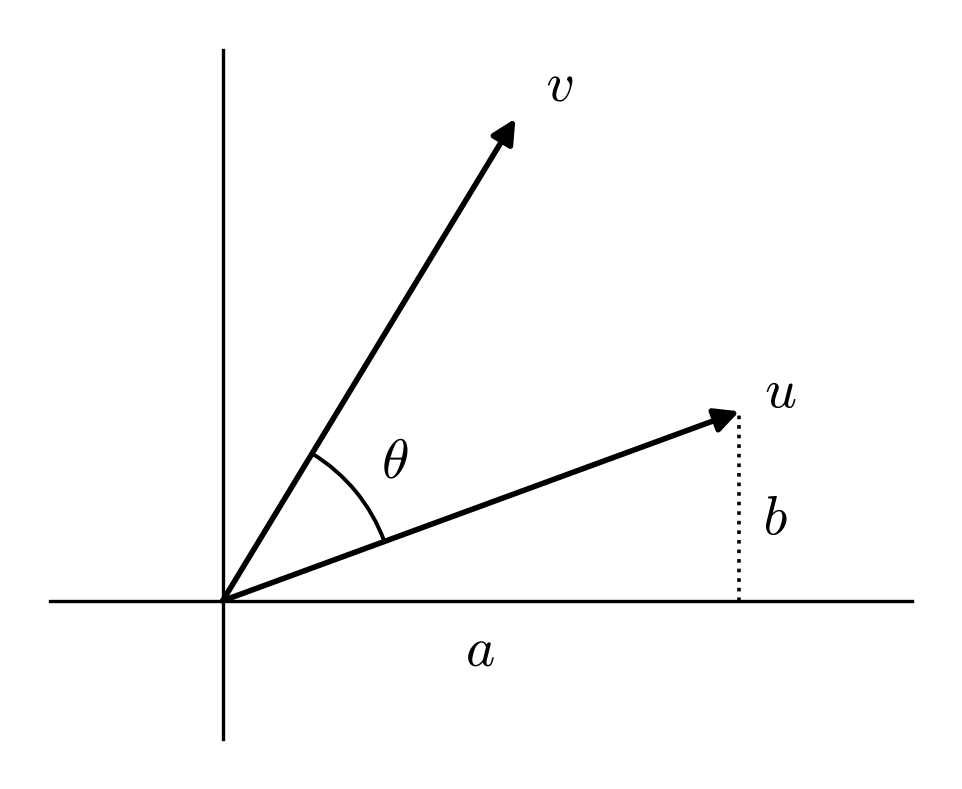
\includegraphics[scale=0.5]{lecture9-fig1-intro}} 
\par\end{center}

במישור אפשר לדבר על שלושה דברים:

1( אורך של \L{$u$}: \L{%
\[
|u|=\sqrt{a^{2}+b^{2}}
\]
}%

2( \L{$\theta$} - זווית בין \L{$u$} ל-\L{$v$}.

3( מכפלה סקלרית: \L{%
\[
\langle u,v\rangle=|u|\cdot|v|\cdot\cos\theta
\]
}%

נרצה להגדיר את 1, 2 ו-3 במ\textquotedblright ו כלשהו מעל \L{$\mathbb{F}$}
)\L{$\mathbb{F}=\mathbb{R}$} או \L{$\mathbb{F}=\mathbb{C}$}(.\\

קודם כל, נשים לב שלמעשה מספיק להגדיר רק את )3( ומשם לקבל גם את )1(
ואת )2(: \L{%
\[
|u|\overset{\text{def}}{=}\sqrt{\langle u,u\rangle}
\]
}%
)הזווית בין \L{$u$} לעצמו היא \L{$0$} ו-\L{$\cos0=1$} לכן זה מסתדר(

ועבור \L{$u,v$} שונים מוקטור האפס )כדי שלא נחלק ב-\L{$0$}(: \L{%
\[
\cos\theta\overset{\text{def}}{=}\frac{\langle u,v\rangle}{|u|\cdot|v|}
\]
}%

במישור, הזווית בין שני וקטורים היא בין \L{$0$} ל-\L{$\pi$}, ובתחום
הזה \L{$\cos$} חח\textquotedblright ע, ולכן \L{$\cos\theta$} קובע
את \L{$\theta$}:\L{%
\[
\theta=\arccos\left(\frac{\langle u,v\rangle}{|u|\cdot|v|}\right)
\]
}%

אבל במ\textquotedblright ו כלשהו צריך שהמנה תהיה מספר ממשי בין \L{$-1$}
ל-\L{$1$}.

אם השדה הוא \L{$\mathbb{R}$} זה נובע מאי-שוויון קושי-שוורץ שבסוף
ההרצאה, אבל אם השדה הוא \L{$\mathbb{C}$} אז המנה יכולה להיות לא ממשית
ולא נוכל לקבוע את הזווית כך.\\

זה הרעיון של כל הנושא.

מגדירים רק מכפלה, והיא בהתאמה מגדירה אורך של וקטור וזווית בין שני
וקטורים.

המישור ומכפלה סקלרית זו רק דוגמה אחת של מ\textquotedblright ו ומכפלה.\\

האיורים המצורפים הם כאילו אנחנו ב-\L{$\mathbb{R}^{2}$}.

הם לאינטואיציה בלבד: \L{$u,v$} יכולים להיות גם פונקציות או אופרטורים.

\part{מרחב מכפלה פנימית, נורמה ואורתוגונליות}

\section{הגדרה - מרחב מכפלה פנימית}

מרחב מכפלה פנימית הוא מ\textquotedblright ו \L{$V$} מעל שדה \L{$\mathbb{F}$}
)כאשר \L{$\mathbb{F}=\mathbb{R}$} או \L{$\mathbb{F}=\mathbb{C}$}(
בצירוף מכפלה פנימית על \L{$V$}.

מכפלה פנימית על \L{$V$} היא פונקציה המעתיקה כל זוג סדור \L{$\left(u,v\right)$}
של איברים ב-\L{$V$} למספר \L{$\left\langle u,v\right\rangle \in\mathbb{F}$}
ומקיימת מספר אקסיומות. 

כלומר, זו פונקציה\L{%
\[
\left\langle \_,\_\right\rangle :V\times V\rightarrow\mathbb{F}
\]
}%

אם לא ברור באיזה מרחב מדובר, נכתוב \L{$\left\langle u,v\right\rangle _{V}$}.\\

האקסיומות שהפונקציה צריכה לקיים הן:\\

{\beginL 1\endL}. חיוביות )כאשר בשני הרכיבים נמצא אותו הוקטור(: \L{%
\[
\forall v\in V:\quad\left\langle v,v\right\rangle \geq0_{\mathbb{F}}
\]
}%

{\beginL 2\endL}. ודאות )כאשר בשני הרכיבים נמצא אותו הוקטור, המכפלה
הפנימית מתאפסת אם\textquotedblright ם הוקטור הוא וקטור האפס(:\L{%
\[
\forall v\in V:\quad\left\langle v,v\right\rangle =0_{\mathbb{F}}\iff v=0_{V}
\]
}%

{\beginL 3\endL}. אדיטיביות ברכיב הראשון:\L{%
\[
\forall v,u,w\in V:\quad\left\langle v+u,w\right\rangle =\left\langle v,w\right\rangle +\left\langle u,w\right\rangle 
\]
}%

{\beginL 4\endL}. הומוגניות ברכיב הראשון:\L{%
\[
\forall\alpha\in\mathbb{F},\ \forall v,u\in V:\quad\left\langle \alpha v,u\right\rangle =\alpha\left\langle v,u\right\rangle 
\]
}%

{\beginL 5\endL}. סימטריית צמוד )הרמיטיות(:\L{%
\[
\forall u,v\in V:\quad\left\langle u,v\right\rangle =\overline{\left\langle v,u\right\rangle }
\]
}%

מדובר על הצמוד המרוכב.

האקסיומה הזו אומרת שאם \L{$\langle v,u\rangle=a+ib$} אז \L{$\langle u,v\rangle=a-ib$}

נזכיר שכל מספר ממשי שווה לצמוד המרוכב שלו, אז מעל \L{$\mathbb{R}$}
פשוט מקבלים \L{$\left\langle u,v\right\rangle =\left\langle v,u\right\rangle $}.\\

הפונקציה \L{$\left\langle \_,\_\right\rangle _{V}$} נקראת מכפלה פנימית,
והזוג \L{$(V,\left\langle \_,\_\right\rangle _{V})$} נקרא מרחב מכפלה
פנימית.\\

נשים לב:
\begin{itemize}
\item לא מניחים ש-\L{$V$} ממימד סופי.
\item צריך את ){\beginL 1\endL}( בשביל שנוכל להגדיר אורך של וקטור )שורש
של מספר אי-שלילי(
\item מכפלה סקלרית והמרחב האוקלידי זה מקרה פרטי של מרחב מכפלה פנימית.
\item יבגני דרש גם \L{$V\ne\left\{ 0_{V}\right\} $}. אקסלר לא דורש את זה,
כתבתי כמו אקסלר.
\item אני כתבתי \L{$\left\langle \_,\_\right\rangle $} כי אני חושב שזה
יותר ברור שאלה ממלאי מקום, אבל בד\textquotedblright כ כותבים \L{$\left\langle \cdot,\cdot\right\rangle $}.
\item \L{$\mathbb{C}$} הוא לא שדה סדור, ולכן במבט ראשון האקסיומה הראשונה
היא תמוהה - אין שם יחס סדר. עם זאת, האקסיומה החמישית מבטיחה שיתקיים
\L{%
\[
\left\langle u,u\right\rangle =\overline{\left\langle u,u\right\rangle }
\]
}%
\\
וזה קורה אם\textquotedblright ם \L{$\left\langle u,u\right\rangle \in\mathbb{R}$}.
כלומר אין כאן באמת בעיה.
\end{itemize}

\subsection{הערה - לינאריות ברכיב הראשון}

נקבע וקטור \L{$w\in V$} ונתבונן בפונקציה \L{%
\[
\left\langle \_,w\right\rangle :V\rightarrow\mathbb{F}
\]
}%
לפי האדיטיביות וההומוגניות ברכיב הראשון, זו ה\textquotedblright ל.

\subsection{{]}תוספת שלי{[} משפט: מכפלה פנימית היא אדיטיבית והומוגנית-צמודה ברכיב
השני}

נשתמש בזה בהוכחות בהמשך.

אקסלר הוכיח את זה כחלק ממשפט נוסף על תכונות של מכפלה פנימית.

יהיו \L{$v,u,w\in V$} ו- \L{$\alpha\in\mathbb{F}$}. אז

\L{%
\[
\langle w,v+u\rangle\underset{\left(1\right)}{=}\overline{\langle v+u,w\rangle}\underset{\left(2\right)}{=}\overline{\langle v,w\rangle}+\overline{\langle u,w\rangle}\underset{\left(1\right)}{=}\langle w,v\rangle+\langle w,u\rangle
\]
}%

\L{%
\[
\langle w,\alpha v\rangle\underset{\left(1\right)}{=}\overline{\langle\alpha v,w\rangle}\underset{\left(3\right)}{=}\overline{\alpha}\cdot\overline{\langle v,w\rangle}\underset{\left(1\right)}{=}\overline{\alpha}\langle w,v\rangle
\]
}%

\L{$\left(1\right)$} סימטריית הצמוד

\L{$(2)$} אדיטיביות ברכיב הראשון + צמוד של סכום הוא סכום הצמודים

\L{$(3)$} הומוגניות ברכיב הראשון + צמוד של מכפלה הוא מכפלת הצמודים

\section{הגדרה - נורמה של וקטור}

יהי \L{$(V,\left\langle \cdot,\cdot\right\rangle )$} מרחב מכפלה פנימית
ויהי \L{$v\in V$}.

הנורמה של \L{$v$} היא \L{%
\[
\|v\|\overset{\text{def}}{=}\sqrt{\langle v,v\rangle}
\]
}%

\begin{itemize}
\item אפשר לחשוב על נורמה של וקטור כעל הכללה של \textquotedblleft אורך של
וקטור\textquotedblright .
\item לפי אקסיומת החיוביות זה מוגדר היטב )שורש של מספר אי-שלילי(.
\item לפי אקסיומת הודאות, \L{$\|v\|=0$} אם\textquotedblright ם \L{$v=0_{V}$}.
\end{itemize}

\section{דוגמה - נורמה לפי המכפלה הפנימית הסטנדרטית ב-\L{$\mathbb{R}^{2}$}}

\L{%
\[
V=\mathbb{R}^{2}=\left\{ (x,y)\ \middle|\ x\in\mathbb{R},\ y\in\mathbb{R}\right\} ,\quad\mathbb{F}=\mathbb{R}
\]
}%
\L{%
\[
\mathcal{B}_{V}=(e_{1},e_{2})=\left((1,0),(0,1)\right)
\]
}%
נגדיר \L{%
\[
\langle v,u\rangle\overset{\text{def}}{=}\alpha_{1}\beta_{1}+\alpha_{2}\beta_{2}
\]
}%
כאשר \L{%
\[
v=\alpha_{1}e_{1}+\alpha_{2}e_{2},\quad u=\beta_{1}e_{1}+\beta_{2}e_{2}
\]
}%

חיוביות: ריבוע של מספר ממשי הוא אי-שלילי, ולכן \L{%
\[
\langle v,v\rangle=\alpha_{1}^{2}+\alpha_{2}^{2}\geq0
\]
}%

ודאות: \L{%
\[
\langle v,v\rangle=0\iff\alpha_{1}^{2}+\alpha_{2}^{2}=0\iff\alpha_{1}=\alpha_{2}=0\underset{\left(*\right)}{\iff}v=0_{V}
\]
}%

\L{$\left(*\right)$} לפי יחידות ההצגה לפי בסיס\\

אדיטיביות ברכיב הראשון: \L{%
\begin{align*}
\langle v+u,w\rangle & =\langle(\alpha_{1}e_{1}+\alpha_{2}e_{2})+(\beta_{1}e_{1}+\beta_{2}e_{2}),\ \gamma_{1}e_{1}+\gamma_{2}e_{2}\rangle\\
 & =\langle\underset{\tilde{\alpha_{1}}}{(\alpha_{1}+\beta_{1})}e_{1}+\underset{\tilde{\alpha_{2}}}{(\alpha_{2}+\beta_{2})}e_{2},\ \underset{\tilde{\beta_{1}}}{\gamma_{1}}e_{1}+\underset{\tilde{\beta_{2}}}{\gamma_{2}}e_{2}\rangle\\
 & \underset{(**)}{=}\underset{\tilde{\alpha_{1}}\tilde{\beta_{1}}}{(\alpha_{1}+\beta_{1})\gamma_{1}}+(\alpha_{2}+\beta_{2})\gamma_{2}\\
 & =(\alpha_{1}\gamma_{1}+\alpha_{2}\gamma_{2})+(\beta_{1}\gamma_{1}+\beta_{2}\gamma_{2})\\
 & \underset{(**)}{=}\langle v,w\rangle+\langle u,w\rangle
\end{align*}
}%

\L{$(**)$} לפי ההגדרה של המכפלה הפנימית הזאת\\

הומוגניות ברכיב הראשון: \L{%
\begin{align*}
\langle cv,u\rangle & =\langle c(\alpha_{1}e_{1}+\alpha_{2}e_{2}),\ \beta_{1}e_{1}+\beta_{2}e_{2}\rangle\\
 & =\langle(c\alpha_{1})e_{1}+(c\alpha_{2})e_{2},\ \beta_{1}e_{1}+\beta_{2}e_{2}\rangle\\
 & \underset{(**)}{=}(c\alpha_{1})\beta_{1}+(c\alpha_{2})\beta_{2}\\
 & =c(\alpha_{1}\beta_{1}+\alpha_{2}\beta_{2})\\
 & \underset{(**)}{=}c\langle v,u\rangle
\end{align*}
}%

סימטריית צמוד:\L{%
\[
\langle u,v\rangle=\beta_{1}\alpha_{1}+\beta_{2}\alpha_{2}\underset{\left(***\right)}{=}\alpha_{1}\beta_{1}+\alpha_{2}\beta_{2}=\langle v,u\rangle\underset{\left(****\right)}{=}\overline{\langle v,u\rangle}
\]
}%

\L{$\left(***\right)$} כפל ממשיים הוא חילופי

\L{$\left(****\right)$} מספר ממשי שווה לצמוד שלו\\

כל חמש האקסיומות מתקיימות, ולכן זו מכפלה פנימית.\\

אצל אקסלר, כאשר מדובר על \L{$\mathbb{F}^{n}$} ולא מגדירים מכפלה פנימית
מפורשות, ברירת המחדל היא המכפלה הפנימית הסטנדרטית )הוא קורא לה \textquotedblleft המכפלה
הפנימית האוקלידית\textquotedblright (.

אפשר להסיק מכך שזו מכפלה פנימית שניתקל בה הרבה.\\

לפי הגדרת הנורמה: \L{%
\[
\|u\|=\sqrt{\langle u,u\rangle}=\sqrt{\beta_{1}^{2}+\beta_{2}^{2}}
\]
}%
\L{%
\[
\|v\|=\sqrt{\langle v,v\rangle}=\sqrt{\alpha_{1}^{2}+\alpha_{2}^{2}}
\]
}%
וזה תואם ל-\textquotedblright אורך\textquotedblright{} שאנחנו מכירים
מהמישור האוקלידי.

\subsection{השוואה למכפלה הסקלרית מההקדמה}

נוכיח שהמכפלה מההקדמה, \L{$\|v\|\cdot\|u\|\cdot\cos\theta$}, שווה
ל- \L{$\langle v,u\rangle$}.

נסמן ב- \L{$\psi$} את הזווית בין \L{$v$} לציר ה-\L{$x$} וב- \L{$\varphi$}
את הזווית בין \L{$u$} לציר ה-\L{$x$}. \\

\begin{center}
\L{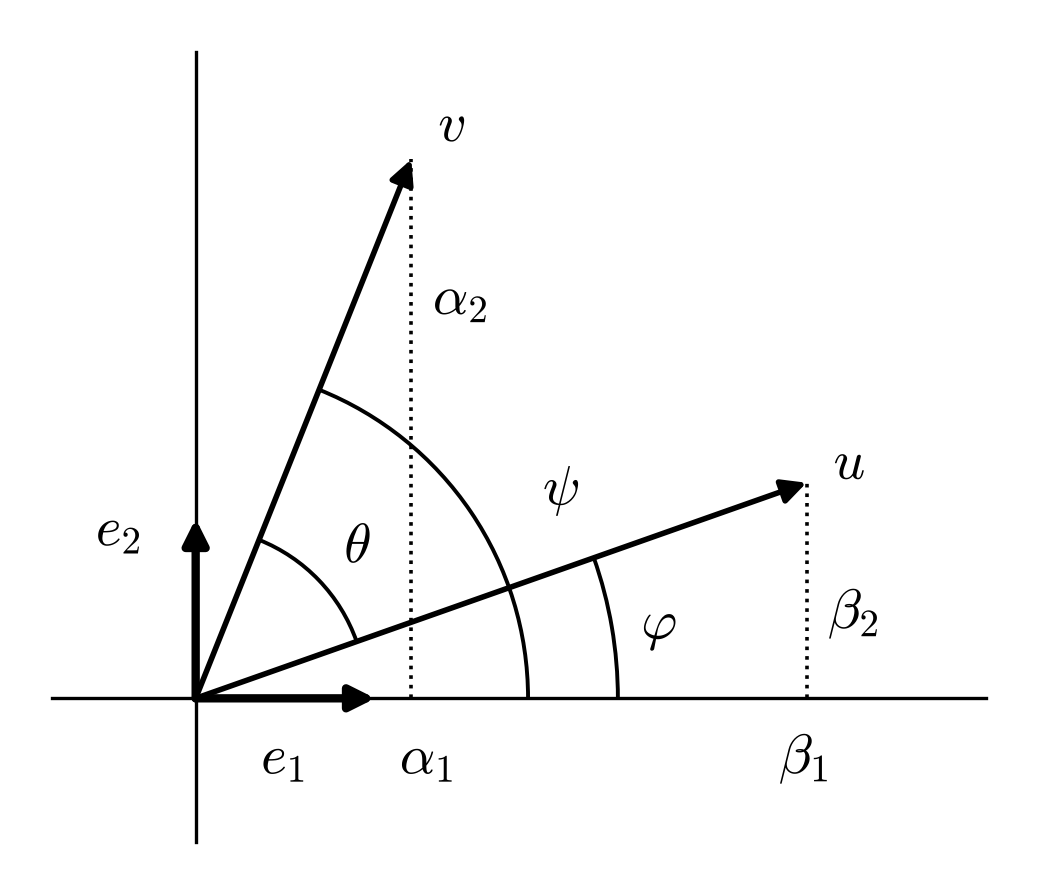
\includegraphics[scale=0.5]{lecture9-fig2-R2-angles}} 
\par\end{center}

אז הזווית בין \L{$u$} ל-\L{$v$} היא \L{%
\[
\theta=\psi-\varphi
\]
}%
ומתקיים\L{%
\[
\|v\|\cos\psi=\alpha_{1},\quad\|v\|\sin\psi=\alpha_{2},\quad\|u\|\cos\varphi=\beta_{1},\quad\|u\|\sin\varphi=\beta_{2}
\]
}%

לכן \L{%
\begin{align*}
\|v\|\cdot\|u\|\cdot\cos\theta & =\|v\|\cdot\|u\|\cdot\cos(\psi-\varphi)\\
 & =\|v\|\cdot\|u\|\cdot\left(\cos\psi\cos\varphi+\sin\psi\sin\varphi\right)\\
 & =\|v\|\cdot\|u\|\cdot\cos\psi\cos\varphi+\|v\|\cdot\|u\|\cdot\sin\psi\sin\varphi\\
 & =\left(\|v\|\cdot\cos\psi\right)\cdot\left(\|u\|\cdot\cos\varphi\right)+\left(\|v\|\cdot\sin\psi\right)\cdot\left(\|u\|\cdot\sin\varphi\right)\\
 & =\alpha_{1}\cdot\beta_{1}+\alpha_{2}\cdot\beta_{2}\\
 & =\langle v,u\rangle
\end{align*}
}%
כנדרש.\\

\begin{itemize}
\item קיבלנו שההגדרה הכללית לא סותרת את מה שמכירים מבית הספר.
\item במ\textquotedblright ו כללי מגדירים הכל בעזרת בסיס וקואורדינטות, ובמקרה
הזה מקבלים אותו דבר.
\item זו לא הדרך היחידה להגדיר מכפלה פנימית על \L{$\mathbb{R}^{2}$}.
\item ההכללה חזקה מאוד, כי יש מ\textquotedblright ו של פונקציות, של מטריצות
ושל ה\textquotedblright ל.
\item בפרט, ה\textquotedblright ל היא וקטור במרחב וקטורי מסוים, ולכן בהמשך
נגיע גם לנורמה של ה\textquotedblright ל.
\end{itemize}

\section{הגדרות: וקטורים מאונכים, רשימה אורתוגונלית, רשימה אורתונורמלית}

יהי \L{$(V,\left\langle \cdot,\cdot\right\rangle )$} מרחב מכפלה פנימית
מעל שדה \L{$\mathbb{F}$} )כאשר \L{$\mathbb{F}=\mathbb{R}$} או \L{$\mathbb{F}=\mathbb{C}$}(.

\subsection{הגדרה: וקטורים מאונכים}

יהיו \L{$u,v\in V$}. אם \L{$\left\langle u,v\right\rangle =0$} נאמר
ש-\L{$u$} ו-\L{$v$} מאונכים ונסמן \L{$u\bot v$}.

נאמר גם ש-\L{$u$} ו-\L{$v$} אורתוגונליים )מאונכים זו המקבילה בעברית(.

\subsection{הגדרה: רשימה אורתוגונלית}

תהי \L{$S=\left(v_{1},\dots,v_{n}\right)$} רשימה של וקטורים מ-\L{$V$}.

הרשימה נקראת אורתוגונלית אם\L{%
\[
\forall1\le i,j\le n:\quad v_{i}\ne0_{V}\quad\wedge\quad\left(i\ne j\Rightarrow\left\langle v_{i},v_{j}\right\rangle =0\right)
\]
}%

זה שקול ל-\L{%
\[
\forall1\le i,j\le n:\quad\begin{cases}
\left\langle v_{i},v_{j}\right\rangle =0 & i\ne j\\
\left\langle v_{i},v_{j}\right\rangle \ne0 & i=j
\end{cases}
\]
}%

\subsection{הגדרה: רשימה אורתונורמלית}

תהי \L{$S=\left(v_{1},\dots,v_{n}\right)$} רשימה של וקטורים מ-\L{$V$}.

הרשימה נקראת אורתונורמלית אם היא אורתוגונלית וגם\L{%
\[
\forall1\le i\le n:\quad\left|\left|v_{i}\right|\right|=1
\]
}%

זה שקול ל-\L{%
\[
\forall1\le i,j\le n:\quad\left\langle v_{i},v_{j}\right\rangle =\begin{cases}
0 & i\ne j\\
1 & i=j
\end{cases}
\]
}%

כי \L{$1=\sqrt[]{1}$} לכן \L{$\left|\left|v\right|\right|=1\iff\left\langle v,v\right\rangle =1$}.\\

וקטור האפס אורתוגונלי לכל וקטור:\L{%
\[
\left\langle 0_{V},v\right\rangle =0\cdot\left\langle 0_{V},v\right\rangle =0
\]
}%
 אבל הוא לא אורתונורמלי, כי הנורמה שלו היא \L{$0$} ולא \L{$1$}.

\subsection{דוגמה - \L{$e_{1},e_{2}$} ב-\L{$\mathbb{R}^{2}$}}

בדוגמה שראינו, הוקטורים \L{$e_{1},e_{2}$} אורתונורמליים.

\L{%
\[
e_{1}=1\cdot e_{1}+0\cdot e_{2},\quad e_{2}=0\cdot e_{1}+1\cdot e_{2}
\]
}%
ולכן \L{%
\[
\langle e_{1},e_{2}\rangle=1\cdot0+0\cdot1=0,\quad\|e_{1}\|=\sqrt{1^{2}+0^{2}}=1,\quad\|e_{2}\|=\sqrt{0^{2}+1^{2}}=1
\]
}%

\textquotedblleft אורתו\textquotedblright{} פירושו מאונכים, ו-\textquotedblright נורמליים\textquotedblright{}
פירושו מנורמלים לאורך \L{$1$}. 

לכן הדוגמה הזאת היא המחשה מצויינת.

כל רשימה אורתונורמלית היא \textquotedblleft מערכת צירים\textquotedblright{}
כזו, אולי מסובבת, שבה לכל ציר יש אותה יחידת מידה והצירים לא נוטים
אחד כלפי השני.

\part{דוגמאות למרחבי מכפלה פנימית}

\section{דוגמה - \L{$\mathbb{R}^{n}$} עם המכפלה הפנימית הסטנדרטית}

\L{%
\[
V=\mathbb{R}^{n}
\]
}%
\L{%
\[
\mathcal{B}_{V}=\left(\underset{e_{1}}{\underbrace{\begin{pmatrix}1\\
0\\
\dots\\
0
\end{pmatrix}}},\underset{e_{2}}{\underbrace{\begin{pmatrix}0\\
1\\
\dots\\
0
\end{pmatrix}}},\dots,\underset{e_{n}}{\underbrace{\begin{pmatrix}0\\
0\\
\dots\\
1
\end{pmatrix}}}\right)
\]
}%
נגדיר \L{%
\[
\langle v,u\rangle\overset{\text{def}}{=}\alpha_{1}\beta_{1}+\dots+\alpha_{n}\beta_{n}
\]
}%
כאשר \L{%
\[
v=\alpha_{1}e_{1}+\dots+\alpha_{n}e_{n}
\]
}%
\L{%
\[
u=\beta_{1}e_{1}+\dots+\beta_{n}e_{n}
\]
}%
אז \L{%
\[
\|v\|=\sqrt{\alpha_{1}^{2}+\dots+\alpha_{n}^{2}}
\]
}%

\section{דוגמה - \L{$\mathbb{C}^{n}$} עם המכפלה הפנימית הסטנדרטית}

\L{%
\[
V=\mathbb{C}^{n}
\]
}%
\L{%
\[
\mathcal{B}_{V}=\left(\underset{e_{1}}{\underbrace{\begin{pmatrix}1\\
0\\
\dots\\
0
\end{pmatrix}}},\underset{e_{2}}{\underbrace{\begin{pmatrix}0\\
1\\
\dots\\
0
\end{pmatrix}}},\dots,\underset{e_{n}}{\underbrace{\begin{pmatrix}0\\
0\\
\dots\\
1
\end{pmatrix}}}\right)
\]
}%
נגדיר \L{%
\[
\langle v,u\rangle\overset{\text{def}}{=}\alpha_{1}\overline{\beta_{1}}+\dots+\alpha_{n}\overline{\beta_{n}}
\]
}%
כאשר \L{%
\[
v=\alpha_{1}e_{1}+\dots+\alpha_{n}e_{n}
\]
}%
\L{%
\[
u=\beta_{1}e_{1}+\dots+\beta_{n}e_{n}
\]
}%
לכל \L{$z\in\mathbb{C}$} מתקיים \L{$z\overline{z}=|z|^{2}$}, ולכן
\L{%
\[
\|v\|=\left(\langle v,v\rangle\right)^{\frac{1}{2}}=\left(\alpha_{1}\overline{\alpha_{1}}+\dots+\alpha_{n}\overline{\alpha_{n}}\right)^{\frac{1}{2}}=\left(|\alpha_{1}|^{2}+\dots+|\alpha_{n}|^{2}\right)^{\frac{1}{2}}
\]
}%
בנוסף, לכל \L{$i,j\in\{1,\dots,n\}$}: \L{%
\[
\langle e_{i},e_{j}\rangle=\begin{cases}
0 & i\neq j\\
1 & i=j
\end{cases}
\]
}%
אז הרשימה \L{$(e_{1},\dots,e_{n})$} אורתונורמלית.

\section{דוגמה - מרחב המטריצות \L{$\text{Mat}(n\times m,\mathbb{C})$}}

\L{%
\[
V=\text{Mat}(n\times m,\mathbb{C})=\left\{ A=\begin{pmatrix}a_{1,1} & \cdots & a_{1,m}\\
\vdots &  & \vdots\\
a_{n,1} & \cdots & a_{n,m}
\end{pmatrix}\ \middle|\ a_{i,j}\in\mathbb{C}\right\} ,\quad\mathbb{F}=\mathbb{C}
\]
}%

\subsection{מטריצה צמודה}

נניח כי \L{%
\[
A=\begin{pmatrix}a_{1,1} & a_{1,2} & \cdots & a_{1,m}\\
a_{2,1} & a_{2,2} & \cdots & a_{2,m}\\
\vdots &  &  & \vdots\\
a_{n,1} & a_{n,2} & \cdots & a_{n,m}
\end{pmatrix}\in\text{Mat}(n\times m,\mathbb{C})
\]
}%
אז \L{%
\[
A^{*}\overset{\text{def}}{=}\begin{pmatrix}\overline{a_{1,1}} & \overline{a_{2,1}} & \cdots & \overline{a_{n,1}}\\
\overline{a_{1,2}} & \overline{a_{2,2}} & \cdots & \overline{a_{n,2}}\\
\vdots &  &  & \vdots\\
\overline{a_{1,m}} & \overline{a_{2,m}} & \cdots & \overline{a_{n,m}}
\end{pmatrix}\in\text{Mat}(m\times n,\mathbb{C})
\]
}%
)כאשר \L{$\overline{z}=\alpha-i\beta$} עבור \L{$z=\alpha+i\beta$}(.\\

מקבלים את \L{$A^{*}$} בשני שלבים.

קודם מחליפים שורות ועמודות )העמודה הראשונה של \L{$A$} הופכת לשורה
הראשונה, וכן הלאה. דהיינו, עושים טרנספוז(, ואחר כך לוקחים בכל מקום
צמוד מרוכב.

\L{$A$} בגודל \L{$n\times m$} ו-\L{$A^{*}$} בגודל \L{$m\times n$},
ולכן אפשר לכפול אותן זו בזו משני הצדדים.

\subsection{עקבה \L{$(\text{Trace})$}}

תהי \L{%
\[
Q=\begin{pmatrix}q_{1,1} & \cdots & q_{1,N}\\
\vdots &  & \vdots\\
q_{N,1} & \cdots & q_{N,N}
\end{pmatrix}\in\text{Mat}(N\times N,\mathbb{F})
\]
}%
נגדיר \L{%
\[
\text{Trace}(Q)\overset{\text{def}}{=}\sum_{i=1}^{N}q_{i,i}
\]
}%

כלומר סכום איברי האלכסון.

כותבים גם \L{$\text{Tr}(Q)$}.

\subsection{דוגמה לשני הסימונים}

\L{%
\[
A=\begin{pmatrix}1 & -i\\
1+2i & -1
\end{pmatrix}
\]
}%
\L{%
\[
A^{*}=\begin{pmatrix}1 & 1-2i\\
i & -1
\end{pmatrix}
\]
}%
\L{%
\[
\text{Tr}(A)=1+(-1)=0
\]
}%

\subsection{הגדרה - מכפלה פנימית של מטריצות}

נניח כי \L{%
\[
A,B\in\text{Mat}(n\times m,\mathbb{C})=V
\]
}%
נגדיר \L{%
\[
\langle A,B\rangle\overset{\text{def}}{=}\text{Trace}(B^{*}\cdot A)
\]
}%

המכפלה \L{$B^{*}A$} היא בגודל \L{$m\times m$}, ולכן ה-\L{$\text{Trace}$}
שלה מוגדר.

לוקחים \L{$B^{*}$} ולא \L{$A^{*}$} כדי שתהיה לינאריות לפי \L{$A$},
הרכיב הראשון. 

\subsection{דוגמה: \L{$n=m=2$}}

נניח כי \L{%
\[
A=\begin{pmatrix}a_{1,1} & a_{1,2}\\
a_{2,1} & a_{2,2}
\end{pmatrix},\quad B=\begin{pmatrix}b_{1,1} & b_{1,2}\\
b_{2,1} & b_{2,2}
\end{pmatrix}
\]
}%
אז \L{%
\[
B^{*}=\begin{pmatrix}\overline{b_{1,1}} & \overline{b_{2,1}}\\
\overline{b_{1,2}} & \overline{b_{2,2}}
\end{pmatrix}
\]
}%
\L{%
\begin{align*}
\text{Trace}(B^{*}A) & =\text{Trace}\left(\begin{pmatrix}\overline{b_{1,1}} & \overline{b_{2,1}}\\
\overline{b_{1,2}} & \overline{b_{2,2}}
\end{pmatrix}\begin{pmatrix}a_{1,1} & a_{1,2}\\
a_{2,1} & a_{2,2}
\end{pmatrix}\right)\\
 & =\text{Trace}\left(\begin{pmatrix}\overline{b_{1,1}}a_{1,1}+\overline{b_{2,1}}a_{2,1} & \overline{b_{1,1}}a_{1,2}+\overline{b_{2,1}}a_{2,2}\\
\overline{b_{1,2}}a_{1,1}+\overline{b_{2,2}}a_{2,1} & \overline{b_{1,2}}a_{1,2}+\overline{b_{2,2}}a_{2,2}
\end{pmatrix}\right)\\
 & =a_{1,1}\overline{b_{1,1}}+a_{2,1}\overline{b_{2,1}}+a_{1,2}\overline{b_{1,2}}+a_{2,2}\overline{b_{2,2}}
\end{align*}
}%
אם \L{$B=A$} נקבל \L{%
\[
\|A\|=\sqrt{|a_{1,1}|^{2}+|a_{2,1}|^{2}+|a_{1,2}|^{2}+|a_{2,2}|^{2}}
\]
}%

כלומר, כדי לחשב נורמה של מטריצה בממ\textquotedblright פ הזה, לוקחים
כל איבר, מחשבים את הערך המוחלט שלו בריבוע, מחברים הכל ולוקחים שורש.

\subsection{המקרה הכללי}

האיבר במקום \L{$(i,j)$} של \L{$B^{*}$} הוא \L{$\overline{b_{j,i}}$},
ולכן האיבר במקום \L{$(i,i)$} של \L{$B^{*}A$} הוא \L{$\underset{j=1}{\overset{n}{\sum}}\overline{b_{j,i}}a_{j,i}$}.

ה-\L{$\text{Trace}$} הוא הסכום של האיברים האלה על \L{$i\in\{1,\dots,m\}$}.
\L{%
\[
\langle A,B\rangle=\text{Tr}(B^{*}A)=\sum_{j=1}^{n}\sum_{i=1}^{m}\overline{b_{j,i}}a_{j,i}
\]
}%
\L{%
\[
\|A\|^{2}=\sum_{j=1}^{n}\sum_{i=1}^{m}\overline{a_{j,i}}a_{j,i}=\sum_{j=1}^{n}\sum_{i=1}^{m}|a_{j,i}|^{2}
\]
}%

עבור \L{$n=m=1$} מקבלים שהנורמה היא הערך המוחלט של מספר מרוכב.

\section{דוגמה - פונקציות רציפות \L{$C[0,1]$}}

\L{%
\[
C[0,1]=V=\left\{ f:[0,1]\rightarrow\mathbb{R}\ \middle|\ f\text{ is continuous}\right\} ,\quad\mathbb{F}=\mathbb{R}
\]
}%
נגדיר \L{%
\[
\langle f,g\rangle\overset{\text{def}}{=}\int_{0}^{1}f(x)g(x)dx
\]
}%
)אינטגרל רימן(

אז \L{%
\[
\|f\|=\sqrt{\int_{0}^{1}f^{2}(x)dx}
\]
}%
ניתן לבדוק כי זה מרחב מכפלה פנימית )לא נוכיח(.\\

\begin{itemize}
\item זו דוגמה למרחב שאינו ממימד סופי.
\item גם כאן אפשר לדבר על פונקציות אורתוגונליות )כאשר האינטגרל שווה ל-\L{$0$}(
ועל פונקציות אורתונורמליות )כאשר בנוסף הנורמות שוות ל-\L{$1$}(.
\item אחת המוטיבציות של הנושא היא להבין מהי נורמה של אופרטור, ומה המשמעות
של \textquotedblleft אופרטור אחד גדול מאופרטור אחר\textquotedblright .
\item זה נושא נפרד שנגיע אליו בהמשך.
\end{itemize}

\part{משפט פיתגורס ואי-שוויון קושי-שוורץ}

\section{משפט פיתגורס במרחבי מכפלה פנימית}

יהי \L{$(V,\left\langle \cdot,\cdot\right\rangle )$} מרחב מכפלה פנימית
מעל \L{$\mathbb{F}$} )כאשר \L{$\mathbb{F}=\mathbb{C}$} או \L{$\mathbb{F}=\mathbb{R}$}(
ויהיו \L{$u,v\in V$} כך ש- \L{$\langle u,v\rangle=0$}. אז \L{%
\[
\|u+v\|^{2}=\|u\|^{2}+\|v\|^{2}
\]
}%

זו הכללה של משפט פיתגורס המוכר.

במשולש ישר זווית עם ניצבים \L{$a,b$} ויתר \L{$c$} מתקיים \L{$c^{2}=a^{2}+b^{2}$}.

המושג המקביל ל-\textquotedblleft\L{$a$} ניצב ל-\L{$b$}\textquotedblright{}
הוא וקטורים אורתוגונליים, ומתברר שהמשפט נכון בכל מרחב מכפלה פנימית. 
\begin{center}
\L{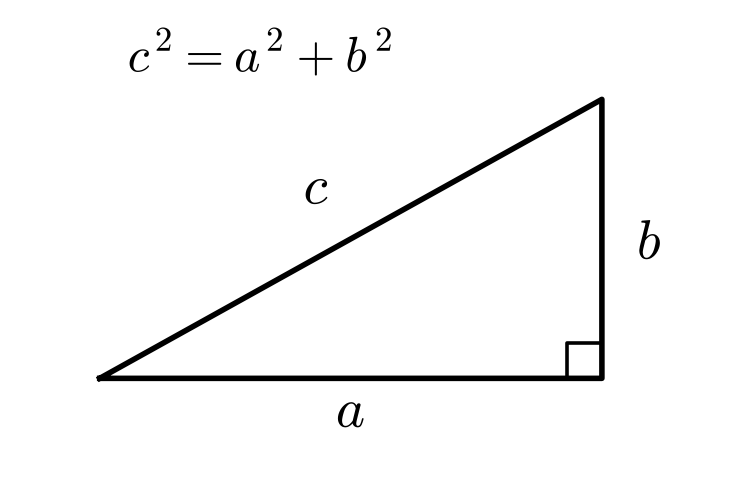
\includegraphics[scale=0.5]{lecture9-fig3-pythagoras}} 
\par\end{center}

יבגני: המשפט הזה לא יינתן במבחן, כי הוא פשוט מדי.
\begin{proof}
נניח כי \L{$\langle u,v\rangle=0$}.

נרצה להוכיח ש- \L{$\|u+v\|^{2}=\|u\|^{2}+\|v\|^{2}$}.

1. לפי הגדרת הנורמה, \L{%
\[
\|u+v\|^{2}=\langle u+v,u+v\rangle
\]
}%

2. נפתח לפי האדיטיביות ברכיב הראשון, ואחר כך לפי האדיטיביות ברכיב
השני: \L{%
\begin{align*}
\langle u+v,u+v\rangle & =\langle u,u+v\rangle+\langle v,u+v\rangle\\
 & =\langle u,u\rangle+\langle u,v\rangle+\langle v,u\rangle+\langle v,v\rangle
\end{align*}
}%

3. לפי ההנחה \L{$\langle u,v\rangle=0$}, ולפי סימטריית הצמוד: \L{%
\[
\langle v,u\rangle=\overline{\langle u,v\rangle}=\overline{0}=0
\]
}%

4. מ-1, 2, 3 נקבל \L{%
\[
\|u+v\|^{2}=\langle u,u\rangle+\langle v,v\rangle+\underset{=0}{\underbrace{\langle u,v\rangle}}+\underset{=0}{\underbrace{\langle v,u\rangle}}=\|u\|^{2}+\|v\|^{2}
\]
}%
כנדרש. 
\end{proof}

\section{משפט אי-שוויון קושי-שוורץ}

זה אחד המשפטים היפים והמפורסמים.

יהי \L{$(V,\left\langle \cdot,\cdot\right\rangle )$} מרחב מכפלה פנימית
מעל \L{$\mathbb{F}$} )כאשר \L{$\mathbb{F}=\mathbb{C}$} או \L{$\mathbb{F}=\mathbb{R}$}(
ויהיו \L{$u,v\in V$}. אז:

)א( \L{%
\[
\left|\langle u,v\rangle\right|\leq\|u\|\cdot\|v\|
\]
}%

)ב( אם \L{%
\[
\left|\langle u,v\rangle\right|=\|u\|\cdot\|v\|
\]
}%
וגם \L{%
\[
u\neq0_{V},\quad v\neq0_{V}
\]
}%
אז קיים \L{$\alpha\in\mathbb{F}$} כך ש- \L{%
\[
u=\alpha v
\]
}%

גרסה חזקה יותר של )ב( שנוכיח בהמשך: \L{%
\[
\left|\langle u,v\rangle\right|=\|u\|\cdot\|v\|
\]
}%

אם\textquotedblright ם \L{$u$} ו-\L{$v$} תלויים לינארית. \\

הערות מיבגני:
\begin{itemize}
\item זה משפט רציני יותר, והוא כן מופיע במבחן מדי פעם.
\item מעכשיו השדה הוא תמיד \L{$\mathbb{R}$} או \L{$\mathbb{C}$}. המשפטים
על שדה כלשהו הסתיימו בפרק הקודם.
\item זה אחד המשפטים החשובים במתמטיקה בכלל.
\item במרחב האוקלידי אי-השוויון הזה טריוויאלי, ומתברר שהוא נכון בכל מרחב
מכפלה פנימית, ומשתמשים בו כל הזמן.
\end{itemize}

\subsection{הערה - \textquotedblleft קוסינוס\textquotedblright{} במרחב מכפלה פנימית}

מ-)א( נובע שלכל שני וקטורים \L{$v,u\in V\setminus\left\{ 0_{V}\right\} $}
מתקיים\L{%
\[
\frac{\left|\langle u,v\rangle\right|}{\|u\|\cdot\|v\|}\leq1
\]
}%

זו אחת מהסיבות שהמשפט הזה חשוב לנו.

בהקדמה רצינו להגדיר את הקוסינוס כמכפלה חלקי מכפלת האורכים, וקוסינוס
חייב להיות בערכו המוחלט לכל היותר \L{$1$}.

לפי )א( זה מתקיים, ולכן אפשר לדבר על \textquotedblleft קוסינוס\textquotedblright{}
כללי, אפילו בין שתי מטריצות.\\

\subsection{הוכחה של )א(}

באיור: \L{$u$} הוא סכום של \L{$av$}, וקטור בכיוון של \L{$v$}, ושל
\L{$w$}, וקטור שניצב ל-\L{$v$}. 
\begin{center}
\L{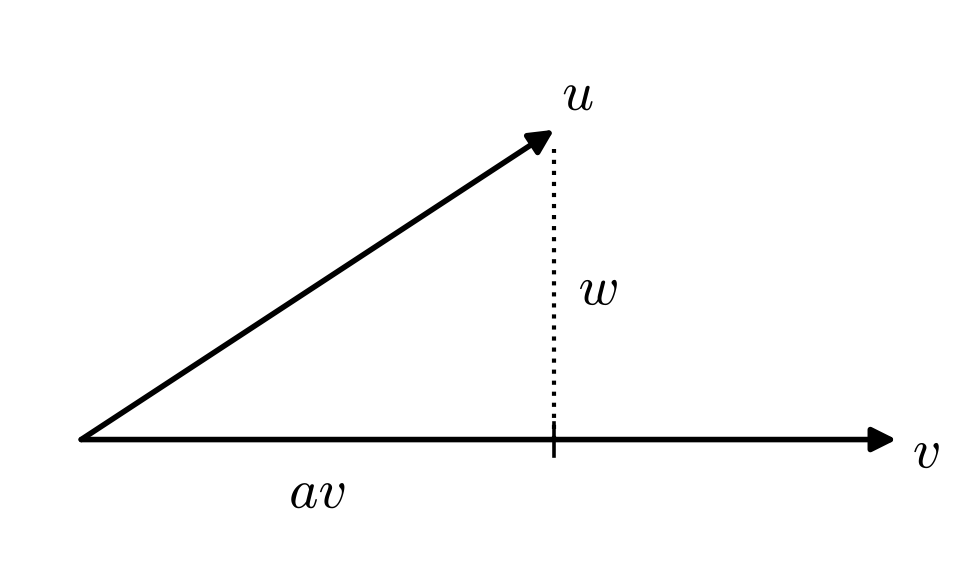
\includegraphics[scale=0.5]{lecture9-fig4-cauchy-schwarz}}\\
\par\end{center}

נוכיח ש- \L{%
\[
\left|\langle u,v\rangle\right|\leq\|u\|\cdot\|v\|
\]
}%

\begin{proof}
1. נניח כי \L{$u=0_{V}$} או \L{$v=0_{V}$}. 

לכל \L{$x\in V$}, לפי ההומוגניות ברכיב הראשון, \L{%
\[
\langle0_{V},x\rangle=\langle0\cdot0_{V},x\rangle=0\cdot\langle0_{V},x\rangle=0
\]
}%
ולפי סימטריית הצמוד גם \L{%
\[
\langle x,0_{V}\rangle=\overline{\langle0_{V},x\rangle}=\overline{0}=0
\]
}%
לכן \L{$\langle u,v\rangle=0$}. 

בנוסף, \L{$\|0_{V}\|=\sqrt{\langle0_{V},0_{V}\rangle}=0$}, ולכן גם
\L{$\|u\|\cdot\|v\|=0$}. 

קיבלנו \L{%
\[
\left|\langle u,v\rangle\right|=0=\|u\|\cdot\|v\|
\]
}%
ו-)א( מתקיים.

2. נניח כי \L{%
\[
v\neq0_{V}\quad\wedge\quad u\neq0_{V}
\]
}%
לפי אקסיומת הודאות, \L{$\langle v,v\rangle\neq0$}, כלומר \L{$\|v\|^{2}\neq0$},
ולכן מותר לחלק ב-\L{$\|v\|^{2}$}.

3. יהי \L{$a\in\mathbb{F}$}. 

נבחר \L{$w=u-av\in V$}. אז \L{%
\[
u=av+w
\]
}%
לפי האדיטיביות וההומוגניות ברכיב הראשון: \L{%
\[
\langle u,v\rangle=\langle av+w,v\rangle=a\langle v,v\rangle+\langle w,v\rangle=a\|v\|^{2}+\langle w,v\rangle
\]
}%

4. נבחר \L{%
\[
a=\frac{\langle u,v\rangle}{\|v\|^{2}}
\]
}%
אז \L{%
\[
a\|v\|^{2}=\langle u,v\rangle
\]
}%
ולכן מהשוויון ב-3:\L{%
\[
\langle u,v\rangle=\langle u,v\rangle+\langle w,v\rangle
\]
}%
 \L{%
\[
\langle w,v\rangle=0
\]
}%
כאשר \L{%
\[
w=u-av=u-\frac{\langle u,v\rangle}{\|v\|^{2}}v
\]
}%

5. נחשב את \L{$\|u\|^{2}$}.

לפי 4 והומוגניות-צמודה ברכיב השני, \L{%
\[
\langle w,av\rangle=\overline{a}\langle w,v\rangle=\overline{a}\cdot0=0
\]
}%
כלומר \L{$w$} ו- \L{$av$} אורתוגונליים, ולכן לפי משפט פיתגורס של
מרחבי מכפלה פנימית \L{%
\[
\|av+w\|^{2}=\|av\|^{2}+\|w\|^{2}
\]
}%
בנוסף, \L{%
\[
\|av\|^{2}=\langle av,av\rangle=a\overline{a}\langle v,v\rangle=|a|^{2}\langle v,v\rangle
\]
}%

מכאן\L{%
\[
\left|\left|u\right|\right|^{2}=\left|\left|av+w\right|\right|^{2}=\|av\|^{2}+\|w\|^{2}=|a|^{2}\langle v,v\rangle+\|w\|^{2}
\]
}%
\L{%
\[
\underset{a=\frac{\langle u,v\rangle}{\|v\|^{2}}}{=}\frac{\left|\langle u,v\rangle\right|^{2}}{\|v\|^{4}}\cdot\|v\|^{2}+\|w\|^{2}=\frac{\left|\langle u,v\rangle\right|^{2}}{\|v\|^{2}}+\|w\|^{2}
\]
}%

6. \L{$\|w\|^{2}\geq0$}, ולכן \L{%
\[
\|u\|^{2}\geq\frac{\left|\langle u,v\rangle\right|^{2}}{\|v\|^{2}}
\]
}%
נכפול ב- \L{$\|v\|^{2}>0$} ונקבל \L{%
\[
\left|\langle u,v\rangle\right|^{2}\leq\|u\|^{2}\cdot\|v\|^{2}
\]
}%
שני האגפים אי-שליליים, ולכן אפשר לקחת שורש: \L{%
\[
\therefore\quad\left|\langle u,v\rangle\right|\leq\|u\|\cdot\|v\|
\]
}%
כנדרש.
\end{proof}

\subsection{הוכחה של )ב(}

נניח כי \L{$\left|\langle u,v\rangle\right|=\|u\|\cdot\|v\|$} וגם
\L{$u\neq0_{V}$}, \L{$v\neq0_{V}$}. 

נרצה להוכיח שקיים \L{$\alpha\in\mathbb{F}$} כך ש-\L{$u=\alpha v$}.
\begin{proof}
1. \L{$v\neq0_{V}$} ו-\L{$u\neq0_{V}$}, ולכן שלבים 2 עד 5 בהוכחה
של )א( תקפים עם אותם \L{$a$} ו-\L{$w$}: \L{%
\[
\|u\|^{2}=\frac{\left|\langle u,v\rangle\right|^{2}}{\|v\|^{2}}+\|w\|^{2}
\]
}%

2. מהשוויון ב-1, ומכך ש- \L{$\left\langle w,w\right\rangle =\|w\|^{2}=0$}
אם\textquotedblright ם \L{$w=0_{V}$} )לפי אקסיומת הודאות(: \L{%
\[
w=0_{V}\iff\|u\|^{2}=\frac{\left|\langle u,v\rangle\right|^{2}}{\|v\|^{2}}
\]
}%

3. לפי ההנחה \L{$\left|\langle u,v\rangle\right|^{2}=\|u\|^{2}\cdot\|v\|^{2}$},
כלומר זה אכן מתקיים ונקבל \L{%
\[
w=0_{V}
\]
}%

4. אז \L{%
\[
u-av=0_{V}
\]
}%
\L{%
\[
\therefore\quad u=av
\]
}%
עבור \L{$a\in\mathbb{F}$} מסוים, כנדרש. 
\end{proof}

\subsection{הכיוון השני של )ב( - לא היה בהרצאה}

בהרצאה הוכחנו רק כיוון אחד, ורק עבור וקטורים שונים מוקטור האפס.

הגרסה המלאה, כמו אצל אקסלר: \L{%
\[
\left|\langle u,v\rangle\right|=\|u\|\cdot\|v\|\iff\exists\alpha\in\mathbb{F}\text{ s.t. }u=\alpha v\text{ or }v=\alpha u
\]
}%
כלומר, אם\textquotedblright ם \L{$u,v$} ת\textquotedblright ל.

\subsubsection{כיוון ראשון: שוויון \L{$\Leftarrow$} אחד הוקטורים הוא כפולה של השני
בסקלר}

נניח כי \L{$\left|\langle u,v\rangle\right|=\|u\|\cdot\|v\|$}.

נרצה להוכיח שקיים \L{$\alpha\in\mathbb{F}$} כך ש-\L{$u=\alpha v$}
או \L{$v=\alpha u$}.
\begin{proof}
1. אם \L{$v=0_{V}$}, אז \L{$v=0\cdot u$}, וסיימנו.

2. נניח כי \L{$v\neq0_{V}$}. 

שלבים 3 עד 5 בהוכחה של )א( משתמשים רק בכך ש-\L{$v\neq0_{V}$}, ולכן
ההוכחה של )ב( תקפה גם אם \L{$u=0_{V}$}. 

לפיה \L{%
\[
u=av
\]
}%
כאשר \L{$a=\frac{\langle u,v\rangle}{\|v\|^{2}}\in\mathbb{F}$}, כנדרש. 
\end{proof}

\subsubsection{כיוון שני: אם אחד הוקטורים הוא כפולה של השני בסקלר אז יש שוויון}

נניח שקיים \L{$\alpha\in\mathbb{F}$} כך ש- \L{$u=\alpha v$} או \L{$v=\alpha u$}.

נרצה להוכיח ש- \L{$\left|\langle u,v\rangle\right|=\|u\|\cdot\|v\|$}.
\begin{proof}
1. לכל \L{$x\in V$} ולכל \L{$\beta\in\mathbb{F}$}, כמו בשלב 5 בהוכחה
של )א(, \L{%
\[
\|\beta x\|^{2}=\langle\beta x,\beta x\rangle=\beta\overline{\beta}\langle x,x\rangle=|\beta|^{2}\|x\|^{2}
\]
}%
שני האגפים אי-שליליים, ולכן אפשר לקחת שורש: \L{%
\[
\|\beta x\|=|\beta|\cdot\|x\|
\]
}%

2. אם \L{$u=\alpha v$}, אז \L{%
\[
\left|\langle u,v\rangle\right|=\left|\langle\alpha v,v\rangle\right|\underset{(1)}{=}\left|\alpha\langle v,v\rangle\right|\underset{(2)}{=}|\alpha|\cdot\|v\|^{2}=\left(|\alpha|\cdot\|v\|\right)\cdot\|v\|\underset{(3)}{=}\|\alpha v\|\cdot\|v\|=\|u\|\cdot\|v\|
\]
}%

3. אם \L{$v=\alpha u$}, אז \L{%
\[
\left|\langle u,v\rangle\right|=\left|\langle u,\alpha u\rangle\right|\underset{(4)}{=}\left|\overline{\alpha}\langle u,u\rangle\right|\underset{(2)}{=}|\alpha|\cdot\|u\|^{2}=\left(\left|\alpha\right|\cdot\left|\left|u\right|\right|\right)\cdot\left|\left|u\right|\right|\underset{(3)}{=}\|\alpha u\|\cdot\|u\|=\|u\|\cdot\|v\|
\]
}%

\L{$(1)$} הומוגניות ברכיב הראשון

\L{$(2)$} \L{$\langle x,x\rangle=\|x\|^{2}\geq0$}, ו-\L{$|\overline{\alpha}|=|\alpha|$}

\L{$(3)$} לפי 1

\L{$(4)$} הומוגניות-צמודה ברכיב השני

בשני המקרים קיבלנו שוויון, כנדרש. 
\end{proof}

\part{נספח - מהרשומות של יבגני}

\section{משפט אי-שוויון המשולש}

המשפט הזה לא היה בהרצאה. הוא מופיע ברשומות של יבגני להרצאה הזו.

יהי \L{$(V,\langle\cdot,\cdot\rangle)$} מרחב מכפלה פנימית מעל \L{$\mathbb{F}$}
)כאשר \L{$\mathbb{F}=\mathbb{R}$} או \L{$\mathbb{F}=\mathbb{C}$}(
ויהיו \L{$u,v\in V$}. אז:

)א( \L{%
\[
\|u+v\|\leq\|u\|+\|v\|
\]
}%

)ב( אם \L{%
\[
\|u+v\|=\|u\|+\|v\|
\]
}%
וגם \L{%
\[
u\neq0_{V},\quad v\neq0_{V}
\]
}%
אז קיים \L{$\alpha\in\mathbb{R}$}, \L{$\alpha\geq0$}, כך ש- \L{%
\[
u=\alpha v
\]
}%

גרסה חזקה יותר של )ב( שנוכיח בהמשך: \L{%
\[
\|u+v\|=\|u\|+\|v\|
\]
}%
אם\textquotedblright ם אחד הוקטורים הוא כפולה של השני בסקלר ממשי אי-שלילי.

\subsection{הוכחה של )א(}

נוכיח ש- \L{%
\[
\|u+v\|\leq\|u\|+\|v\|
\]
}%

\begin{proof}
1. כמו בשלבים 1 ו-2 בהוכחת משפט פיתגורס, \L{%
\[
\|u+v\|^{2}=\langle u+v,u+v\rangle=\langle u,u\rangle+\langle u,v\rangle+\langle v,u\rangle+\langle v,v\rangle
\]
}%

2. לפי סימטריית הצמוד \L{$\langle v,u\rangle=\overline{\langle u,v\rangle}$},
ולכל \L{$z\in\mathbb{C}$} מתקיים \L{$z+\overline{z}=2\text{Re}(z)$}.
לכן \L{%
\[
\|u+v\|^{2}=\|u\|^{2}+\|v\|^{2}+2\text{Re}\left(\langle u,v\rangle\right)
\]
}%

3. \L{%
\begin{align*}
\|u\|^{2}+\|v\|^{2}+2\text{Re}\left(\langle u,v\rangle\right) & \underset{(1)}{\leq}\|u\|^{2}+\|v\|^{2}+2\left|\langle u,v\rangle\right|\\
 & \underset{(2)}{\leq}\|u\|^{2}+\|v\|^{2}+2\|u\|\cdot\|v\|\\
 & =\left(\|u\|+\|v\|\right)^{2}
\end{align*}
}%

\L{$(1)$} לכל \L{$z\in\mathbb{C}$} מתקיים \L{$\text{Re}(z)\leq|z|$}

\L{$(2)$} אי-שוויון קושי-שוורץ, )א(

4. מ-2 ו-3 נקבל \L{%
\[
\|u+v\|^{2}\leq\left(\|u\|+\|v\|\right)^{2}
\]
}%
שני האגפים הם ריבועים של מספרים אי-שליליים, ולכן אפשר לקחת שורש: \L{%
\[
\therefore\quad\|u+v\|\leq\|u\|+\|v\|
\]
}%
כנדרש. 
\end{proof}

\subsection{הוכחה של )ב(}

נניח כי \L{$\|u+v\|=\|u\|+\|v\|$} וגם \L{$u\neq0_{V}$}, \L{$v\neq0_{V}$}.

נרצה להוכיח שקיים \L{$\alpha\in\mathbb{R}$}, \L{$\alpha\geq0$},
כך ש- \L{$u=\alpha v$}.
\begin{proof}
1. מההנחה, \L{$\|u+v\|^{2}=\left(\|u\|+\|v\|\right)^{2}$}.

לפי שלבים 2 ו-3 בהוכחה של )א(: \L{%
\[
\|u+v\|^{2}=\|u\|^{2}+\|v\|^{2}+2\text{Re}\left(\langle u,v\rangle\right)\le\|u\|^{2}+\|v\|^{2}+2\left|\langle u,v\rangle\right|\le\|u\|^{2}+2\|u\|\|v\|+\|v\|^{2}=\left(\|u\|+\|v\|\right)^{2}
\]
}%
אבל הביטוי הראשון והביטוי האחרון שווים!

לכן כל הא\textquotedblright ש הם למעשה שוויונות ונקבל בפרט\L{%
\[
\text{Re}\left(\langle u,v\rangle\right)=\left|\langle u,v\rangle\right|
\]
}%
\L{%
\[
\left|\langle u,v\rangle\right|=\|u\|\cdot\|v\|
\]
}%

2. מהשוויון השני, ומכך ש-\L{$u\neq0_{V}$} ו-\L{$v\neq0_{V}$}, לפי
חלק )ב( של אי-שוויון קושי-שוורץ קיים \L{$\alpha\in\mathbb{F}$} כך
ש- \L{$u=\alpha v$}.

3. נציב \L{$u=\alpha v$} בשוויון הראשון.

לפי ההומוגניות ברכיב הראשון, \L{%
\[
\langle\alpha v,v\rangle=\alpha\langle v,v\rangle=\alpha\|v\|^{2}
\]
}%
ו-\L{$\|v\|^{2}$} ממשי ואי-שלילי. לכן \L{%
\[
\text{Re}\left(\langle u,v\rangle\right)=\text{Re}\left(\alpha\|v\|^{2}\right)=\text{Re}(\alpha)\cdot\|v\|^{2}
\]
}%
\L{%
\[
\left|\langle u,v\rangle\right|=\left|\langle\alpha v,v\rangle\right|=\left|\alpha\|v\|^{2}\right|=|\alpha|\cdot\|v\|^{2}
\]
}%

לפי השוויון הראשון משלב 1, \L{$\text{Re}\left(\langle u,v\rangle\right)=\left|\langle u,v\rangle\right|$}.
לכן \L{%
\[
\text{Re}(\alpha)\cdot\|v\|^{2}=\text{Re}\left(\langle u,v\rangle\right)=\left|\langle u,v\rangle\right|=|\alpha|\cdot\|v\|^{2}
\]
}%
\L{%
\[
\therefore\quad\text{Re}(\alpha)\cdot\|v\|^{2}=|\alpha|\cdot\|v\|^{2}
\]
}%

4. \L{$v\neq0_{V}$}, ולכן לפי אקסיומת הודאות \L{$\|v\|^{2}\neq0$}.
מכאן \L{%
\[
\text{Re}(\alpha)=|\alpha|
\]
}%

5. נכתוב \L{$\alpha=x+iy$} כאשר \L{$x,y\in\mathbb{R}$}.

אז\L{%
\[
\text{Re}(\alpha)=x=|\alpha|=\sqrt{x^{2}+y^{2}}
\]
}%

לכן \L{$x\geq0$}, ובהעלאה בריבוע \L{$x^{2}=x^{2}+y^{2}$}, כלומר
\L{$y=0$}. \L{%
\[
\therefore\quad\alpha=x\in\mathbb{R},\quad\alpha\geq0
\]
}%
כנדרש. 
\end{proof}

\subsection{הכיוון השני של )ב( - לא ברשומות ולא בהרצאה}

ברשומות מופיע רק כיוון אחד, ורק עבור וקטורים שונים מוקטור האפס.

הגרסה המלאה, כמו אצל אקסלר: \L{%
\[
\|u+v\|=\|u\|+\|v\|\iff\exists0\le\alpha\in\mathbb{R},\text{ s.t. }u=\alpha v\text{ or }v=\alpha u
\]
}%

\subsubsection{כיוון ראשון: שוויון \L{$\Leftarrow$} אחד הוקטורים הוא כפולה אי-שלילית
של השני}

נניח כי \L{$\|u+v\|=\|u\|+\|v\|$}.

נרצה להוכיח שקיים \L{$0\le\alpha\in\mathbb{R}$}, כך ש- \L{$u=\alpha v$}
או \L{$v=\alpha u$}.
\begin{proof}
1. אם \L{$v=0_{V}$}, אז \L{$v=0\cdot u$}, וסיימנו.

2. אם \L{$u=0_{V}$}, אז \L{$u=0\cdot v$}, וסיימנו.

3. אחרת \L{$u\neq0_{V}$} ו-\L{$v\neq0_{V}$}, ולפי חלק )ב( קיים \L{$\alpha\in\mathbb{R}$},
\L{$\alpha\geq0$}, כך ש-\L{$u=\alpha v$}, כנדרש. 
\end{proof}

\subsubsection{כיוון שני: אם אחד הוקטורים הוא כפולה אי-שלילית של השני אז יש שוויון}

נניח שקיים \L{$0\le\alpha\in\mathbb{R}$}, כך ש- \L{$u=\alpha v$}
או \L{$v=\alpha u$}.

נרצה להוכיח ש- \L{$\|u+v\|=\|u\|+\|v\|$}.
\begin{proof}
1. כפי שראינו בכיוון השני של )ב( בקושי-שוורץ, לכל \L{$x\in V$} ולכל
\L{$\beta\in\mathbb{F}$} מתקיים \L{$\|\beta x\|=|\beta|\cdot\|x\|$}.

בנוסף \L{$\alpha\geq0$}, ולכן \L{$|\alpha|=\alpha$} ו- \L{$|\alpha+1|=\alpha+1$}.

2. אם \L{$u=\alpha v$}, אז \L{$u+v=(\alpha+1)v$}, ולכן \L{%
\[
\|u+v\|=\|(\alpha+1)v\|=(\alpha+1)\|v\|=\alpha\|v\|+\|v\|=\|\alpha v\|+\|v\|=\|u\|+\|v\|
\]
}%

ואם \L{$v=\alpha u$}, אז \L{$u+v=(1+\alpha)u$}, ולכן \L{%
\[
\|u+v\|=\|(1+\alpha)u\|=(1+\alpha)\|u\|=\|u\|+\alpha\|u\|=\|u\|+\|\alpha u\|=\|u\|+\|v\|
\]
}%
כנדרש. 
\end{proof}

\end{document}
